%!TeX TS-program = Lualatex 
%!TeX encoding = UTF-8 Unicode 
%!TeX spellcheck = en-US
%!BIB program = bibtex
%%%%%%%%%%%%%%%%%%%%%%%%%%%%%%%%%%%%%%%%%%%%%%%%%%%%%%%%%%%%%%%%%%%%%
%!TeX TS-program = Lualatex 
%!TeX encoding = UTF-8 Unicode 
%!TeX spellcheck = en-US
%!TEX root = PerrinetBednar15srep.tex
%%%%%%%%%%%%%%%%%%%%%%%%%%%%%%%%%%%%%%%%%%%%%%%%%%%%%%%%%%%%%%%%%%%%%
\newcommand{\AuthorA}{Laurent U.~Perrinet}%
\newcommand{\AuthorB}{James A.~Bednar} %
\newcommand{\AddressA}{Institut de Neurosciences de la Timone \\
CNRS / Aix-Marseille Universit\'e}% - Marseille, France
\newcommand{\LongAddressA}{
Institut de Neurosciences de la Timone (UMR 7289),
Aix Marseille Universit\'e, CNRS \\
%Facult\'e de M\'edecine - B\^atiment Neurosciences,
27, Bd Jean Moulin,
13385 Marseille Cedex 05,
France}
\newcommand{\PhoneA}{+33.491 324 044}%
\newcommand{\AddressB}{Institute for Adaptive and Neural Computation\\
University of Edinburgh}%
\newcommand{\Website}{http://invibe.net/LaurentPerrinet}%
\newcommand{\Email}{Laurent.Perrinet@univ-amu.fr}%
\newcommand{\Title}{Edge co-occurrences can account for rapid categorization of natural versus animal images}% 88 chars <90
\newcommand{\ShortTitle}{Edge co-occurrences categorize natural images}%
\newcommand{\Abstract}{
Making a judgment about the semantic category of a visual scene, such as whether it contains an animal, is typically assumed to involve high-level associative brain areas. Previous explanations require progressively analyzing the scene hierarchically at increasing levels of abstraction, from edge extraction to mid-level object recognition and then object categorization. Here we show that the statistics of edge co-occurrences alone are sufficient to perform a rough yet robust (translation, scale, and rotation invariant) scene categorization. We first extracted the edges from images using a scale-space analysis coupled with a sparse coding algorithm. We then computed the ``association field'' for different categories (natural, man-made, or containing an animal) by computing the statistics of edge co-occurrences. These differed strongly, with animal images having more curved configurations. We show that this geometry alone is sufficient for categorization, and that the pattern of errors made by humans is consistent with this procedure. Because these statistics could be measured as early as the primary visual cortex, the results challenge widely held assumptions about the flow of computations in the visual system. The results also suggest new algorithms for image classification and signal processing that exploit correlations between low-level structure and the underlying semantic category.
}%
\newcommand{\Keywords}{natural scene statistics; edge co-occurrence; good continuation; association field; lateral connections}%
\newcommand{\Acknowledgments}{%
We are very grateful for the reviewers' and editor effort and time to improve this paper. 
L.U.P.\ was supported by EC IP project FP7-269921, ``BrainScaleS'' and 
ANR project "BalaV1" N°ANR-13-BSV4-0014-02. 
Thanks to David Fitzpatrick for allowing J.A.B.\ access to the laboratory 
in which the man-made images were taken. 
Correspondence and requests for materials 
should be addressed to LUP (email:\Email\ )%
\footnote{Code and supplementary material available 
at \url{\Website/Publications/PerrinetBednar15}.}. %
}%
\newcommand{\SignificanceStatement}{%
 Humans can very rapidly judge the category of an image, such as
 whether it contains an animal. Previous theories for this capability
 require hierarchical grouping of low-level edge elements into
 increasingly complex object representations. Here we show that the
 edges alone are sufficient for this judgment, if the patterns of
 co-occurrence between them are taken into account. For instance,
 images with animals tend to have contours that are more highly
 curved. These results suggest that humans could be using low-level
 statistical regularities to drive rapid but accurate high-level
 judgments, and could help improve computer vision systems.
 %% 100 words
}
\newcommand{\Highlights}{%
\begin{itemize}
\item Humans very efficiently judge the category of an image. 
 
\item Previous theories require hierarchical grouping of object representations. 
 
 \item We show that the edges alone are sufficient for this judgment.
 
 \item The pattern of edge co-occurrence is sufficient to categorize an image with an animal. 
 
 \item Humans could be using such low-level statistical regularities to drive decisions.

 \item Future computer vision systems could use such features.

\end{itemize}
}%
%%%%%%%%%%%%%%%%%%%%%%%%%%%%%%%%%%%%%%%%%%
%%%%%%%%%%%%%%%%%%%%%%%%%%%%%%%%%%%%%%%%%%
%%%%%%%%%%%%%%%%%%%%%%%%%%%%%%%%%%%%%%%%%%
%%%%%%%%%%%%%%%%%%%%%%%%%%%%%%%%%%%%%%%%%%
\documentclass{article}%twocolumn, 
%============ graphics ===================
\usepackage{graphicx}% 
\DeclareGraphicsExtensions{.pdf,.png,.jpg}
\graphicspath{{../figures/},{./}}% 
\usepackage[numbers,comma,sort&compress]{natbib} % ,round
%============ hyperref ===================
\usepackage[unicode,linkcolor=blue,citecolor=blue,filecolor=black,urlcolor=blue,pdfborder={0 0 0}]{hyperref}%
\hypersetup{%
pdftitle={\Title},%
pdfauthor={\AuthorA < \Email > \AddressA - \Website; \AuthorB \AddressB },%
pdfkeywords={\Keywords},%
pdfsubject={\Acknowledgments}%
}%
%%%%%%%%%%%% authblk %%%%%%%%%%%%%%%
\usepackage[affil-sl]{authblk}%
\title{\Title}%
\author{\AuthorA \thanks{Correspondence to \Email}}%}
\affil{\AddressA}
\author{\AuthorB } 
\affil{\AddressB}
\renewcommand\Authands{ and }
\date{}
\usepackage{color}
%%%%%%%%%%%% supp %%%%%%%%%%%%%%%
\usepackage{pdfpages}
%%%%%%%%%%%% Her begynner selve dokumentet %%%%%%%%%%%%%%%
\begin{document}%
%% The \maketitle command is necessary to build the title page.
\maketitle%
%%%%%%%%%%%%%%%%%%%%%%%%%%%%%%%%%%%%%%%%%%%%%%%%%%%%%%%%%%%%%%%%
%: abstract
{\bf %\begin{abstract}%
\begin{quote}
%Summary
%
\Abstract
\end{quote}
}%\end{abstract}%
%
\subsection*{Keywords}%
\Keywords%
%
%\subsection*{Significance Statement}%
%\noindent\SignificanceStatement %
\subsection*{Highlights}%
\noindent\Highlights %
%%%%%%%%%%%%%%%%%%%%%%%%%%%%%%%%%%%%%%
\section*{Introduction}% 216 words
%%%%%%%%%%%%%%%%%%%%%%%%%%%%%%%%%%%%%%
Oriented edges in images of natural scenes tend to be aligned in co-linear or co-circular arrangements, 
with lines and smooth curves more common than other possible arrangements of edges. 
The visual system appears to take advantage of this prior knowledge about natural images, 
with human contour detection and grouping performance well predicted 
by such an ``association field''~\citep{Field93} between edge elements. 
\citet{Geisler01} have estimated this prior information available
to the visual system by extracting contours from a database of natural
images, and showed that these statistics could predict behavioral data
from humans in a line completion task.

One possible candidate substrate for implementing an association field in mammals is
the set of long-range lateral connections between neurons in the primary visual cortex (V1), 
which could act to detect contours matching the association field~\citep{Hunt11}. %~\citep{Choe04}
To fill this role, lateral connections would need to be orientation specific 
and aligned along contours~\citep{Hess03}, and
indeed such an arrangement has been found in V1
of the tree shrew~\citep{Bosking97,Hunt11} and the
monkey~\citep{Sincich01}. 
%Such an elementary circuit could serve as the basis of synchronous activation of neurons
%along a contour~\citep{Samonds06}. 
%This circuitry is compatible with the implementation of the ``good continuation law'' of Gestalt psychology applied to co-circular contours in natural images~\citep{Sigman01}. %, and of curvature detection~\citep{Parent89}. % Cichy14 says it may be involved in the processing within the 100-150ms window

In this paper, we show that an association field of this type can be
used for image categorization.  Human performance in tasks like
determining whether an image contains an animal is surprisingly
accurate even at very rapid time scales~\cite{Thorpe96}.  To explain
this rapid process, previous researchers have investigated whether
low-level features could explain human performance in rapid
categorization tasks, but they concluded with general claims that ``it
is very unlikely that human observers could rely on low-level cues''
(\citealp{Serre07},
\href{http://www.pnas.org/content/suppl/2007/03/23/0700622104.DC1/00622Table2.pdf}{SI
  Table 2}), and ``low-level information [alone] cannot explain human
performance'' (\citealp{Drewes11}, p.19).  Here we show that 
alternative low-level cues, namely the association field between edges
represented as early as V1, can achieve image
categorization performance comparable to humans and to previous
hierarchical models of the visual system.  We also show the images
falsely reported as having animals by humans have association fields
strongly resembling those of animal images, suggesting that humans are
making use of this co-occurrence information when performing rapid
image categorizations.


%------------------------------------------------------------------------------------------------%
%: fig:model 1 _ 103 words
\begin{figure}[p]%ht!]%[p!] 
\centering%
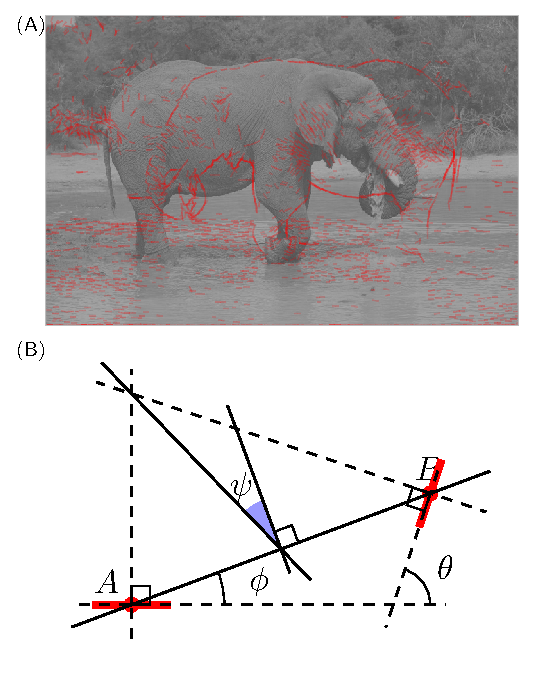
\includegraphics[width=.9\textwidth]{figure_model}%
%%\vspace*{-4cm} 
\caption{ 
$\mathsf{(A)}$ An example image with the list of extracted edges overlaid.  
Each edge is represented by a red line segment which represents its position (center of segment), orientation, and scale (length of segment). 
%The edge's coefficient is represented by its strength (value of segment's color) and phase (hue).
%The image was taken by author J.A.B.
We controlled the quality of the reconstruction from the edge information such
that the residual energy was less than $5\%$.
%a criterion met when identifying 1024 edges per image. 
$\mathsf{(B)}$ The relationship between a reference edge \emph{A} and another
edge \emph{B} can be quantified in terms of the difference between their
orientations $\theta$, 
ratio of scale $\sigma$, %relative to the reference edge, 
distance $d$ between their centers, 
and difference of azimuth (angular location) $\phi$. %
Additionally, we define $\psi=\phi - \theta/2$, which is
symmetric with respect to the choice of the reference edge; 
in particular, $\psi=0$ for co-circular edges. % (see text). 
As in~\citet{Geisler01}, edges outside a central circular mask are discarded in the computation of the statistics to avoid artifacts. 
%
Image credit:~\href{https://commons.wikimedia.org/wiki/File:Elephant_\%28Loxodonta_Africana\%29_05.jpg}{Andrew Shiva, Creative Commons Attribution-Share Alike 3.0 Unported license}.
\label{fig:model} %
 } %
\end{figure} %
%------------------------------%
%{\color{blue}
%%%%%%%%%%%%%%%%%%%%%%%%%%%%%%%%%%%%%%%
\section*{Results} %98 + 235 + 148 = 481
%Categorization using the statistics of edge co-occurrences}%Results: Robust c
%%%%%%%%%%%%%%%%%%%%%%%%%%%%%%%%%%%%%%%
%%%%%%%%%%%%%%%%%%%%%%%%%%%%%%%%%%%%%%%
%%\subsection{Statistics of edges}
%%%%%%%%%%%%%%%%%%%%%%%%%%%%%%%%%%%%%%%
To determine what information edge co-occurences could provide
about image category, we examined how the statistics of
edge co-occurrence vary across three image categories.
The first two consist of the image databases ($600$ images each) used by~\citet{Serre07}, 
which contain either animals at different close-up views in a natural setting (which we call ``animal images''), 
or natural images without animals (which we call ``non-animal natural images''). %.
%\footnote{Publicly available at {\it http://cbcl.mit.edu/software-datasets/serre/SerreOlivaPoggioPNAS07}.}. 
A third database consists of 
self-acquired images from a biology laboratory setting, 
containing $600$ indoor 
views of a man-made indoor environment 
%of furniture, windows, and doors and cages 
in which animals are reared (which we call ``man-made images''). 
These images also do not contain animals, 
but provide a novel set for control purposes. %
%------------------------------------------------------------------------------------------------%
From a sparse representation of oriented edges at different scales, we
define the association field as the four-dimensional histogram of edge
co-occurrences $p(d, \psi, \theta, \sigma)$ (see
definitions in Figure~\ref{fig:model}). %

Computing the Kullback-Leibler (KL) divergence between this
four-dimensio\-nal function and various possible factorizations suggests
that we can consider $p(d,\sigma)$ separately from $p(\psi, \theta)$
(see SI table 1).  The distribution of edge distances and relative scales
$p(d,\sigma)$ proved to be quite similar across the different classes
of images (see SI figure 3), because these variables depend
primarily on the viewpoint and location of the observer rather than on
the objects in the scene.  The remaining two angular parameters
$p(\psi, \theta)$ can be visualized using a ``chevron map'' (see
Figure~\ref{fig:chevrons}), %-C and Figure~\ref{fig:chevrons2}).
which indicates the probability of each possible angular configuration
between edges.  As found in previous work~\citep{Geisler01},
collinear, parallel, and (to some extent) orthogonal configurations
appear more commonly than chance.  Results for other datasets are
broadly similar, but with systematic differences.
Figure~\ref{fig:chevrons2} shows chevron maps for the difference
between the non-animal natural image dataset and the other two datasets.
In particular, images of man-made environments have more collinear
configurations, while images with animals have more highly curved and
converging angles, and fewer collinear or orthogonal configurations.

%------------------------------% 
%: fig:chevrons% 127 words
\begin{figure}%[p]%ht!]%[p!]
\centering{
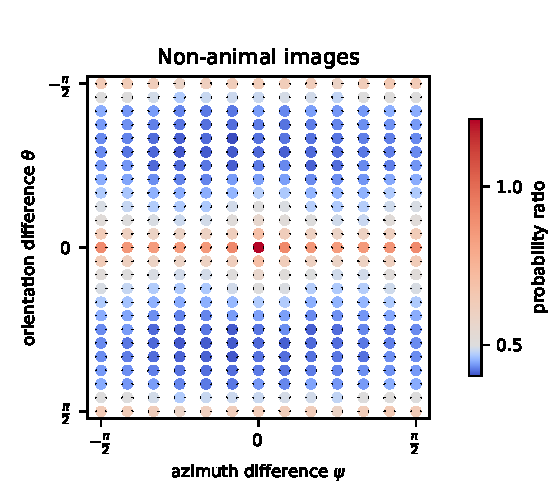
\includegraphics[width=.6\textwidth]{figure_chevrons}%
}
\caption{
The probability distribution function $p(\psi, \theta)$ 
represents the distribution of the different geometrical arrangements of edges' angles, 
which we call a ``chevron map''. 
We show here the histogram for non-animal natural images, 
illustrating the preference for co-linear edge configurations. 
For each chevron configuration, deeper and deeper red circles 
indicate configurations that are more and more likely 
with respect to a uniform prior, % (all configurations equally likely), 
with an average maximum of about $3$ times more likely, 
and deeper and deeper blue circles indicate configurations less likely 
than a flat prior (with a minimum of about $0.8$ times as likely). 
Conveniently, this ``chevron map'' shows in one graph that non-animal natural images 
have on average a preference for co-linear and parallel edges, 
(the horizontal middle axis) and %as seen in Figure~\ref{fig:model}-D, 
orthogonal angles (the top and bottom rows),
along with a slight preference for co-circular configurations (for $\psi=0$ and $\psi=\pm \frac \pi 2$, just above and below the central row).
\label{fig:chevrons}}% 
\end{figure}%
%------------------------------% 
% \showthe\columnwidth
% R2 235 words
To assess these differences 
quantitatively, we built a simple classifier to measure if this representation 
is sufficient to categorize different image categories reliably. 
For each individual image, we constructed a vector of features as either 
%
(FO) the first-order statistics, i.e., the histogram of edge orientations,
(CM) the ``chevron map'' subset of the second-order statistics, (i.e., the two-dimensional histogram of relative orientation and azimuth; as in Figure~\ref{fig:chevrons}), or 
(SO) the full, four-dimensional histogram of second-order statistics (i.e., all four parameters of the edge co-occurrences).
%
  We gathered these vectors for each different class of images and
  tested a standard Support Vector Machine (SVM) classification
  algorithm.  The results of the SVM classifier are reported using an
  F1 score, as in~\citet{Serre07}, which equally weights false
  positive and false negative error rates to fairly assess each
  approach.  Here we used the F1 score to directly compare our method
  to that of~\citet{Serre07}.  This process was cross-validated 20
  times by drawing new training and testing sets.  Using these
  different trials, we could measure the variability of the F1 score.
  The variability was always less than $\approx 4\%$.
  Results are summarized in Figure~\ref{fig:results}.

% R3 148 words
Performance is almost perfect for distinguishing non-animal natural versus
  laboratory (man-made) images, and is still quite high for
  classifying animal images versus non-animal natural images, a much
  more subtle distinction.
This high level of performance is very surprising, given the explicit
claims from~\citet{Serre07} and others that no low-level cue was likely to work well.
Results for the chevron map
confirm that performance of the classifier comes primarily from a geometrical feature 
rather than a viewpoint-dependent feature. % (such as the scale of edges). 
%
% -------------------------------- %
%: fig:chevrons2  83 words
\begin{figure}%[p]%[ht!]
%\centering%
%\hspace*{-0.03\textwidth}%
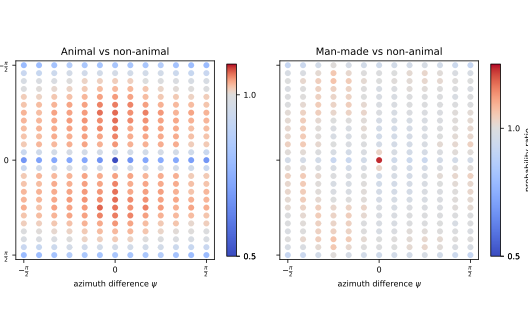
\includegraphics[width=1.\textwidth]{figure_chevrons2}%
%\centering{
%\begin{tikzpicture}
%\node [anchor=south west] (label) at (-1, 0) 
%	{\includegraphics[width=\textwidth]{figure3}};
%\draw (0, 10.75) node {$\mathsf{(A)}$};%
%\draw (9, 10.75) node {$\mathsf{(B)}$};%
%\end{tikzpicture}
%}
%\vspace*{-2cm} 
% 14-06-13_DONE-following-skype  : make colorbars
\caption{%
%{\bf Chevron maps in man-made and animal images compared to the `natural' set.} 
As for Figure~\ref{fig:chevrons}, we show the probability of edge
configurations as chevron maps for two databases (man-made, animal).
Here, we show the ratio of histogram counts relative to that of the
non-animal natural image dataset.  Deeper and deeper red circles
indicate configurations that are more and more likely (and blue
respectively less likely)
with respect to the histogram computed for non-animal images.  
In the left plot, the animal
images exhibit relatively more circular continuations and converging angles (red
chevrons in the central vertical axis) relative to non-animal natural images, 
at the expense of co-linear, parallel, and orthogonal configurations (blue circles along the middle horizontal axis). %
The man-made images have strikingly more co-linear features (central circle), which reflects the prevalence of long, straight lines in the cage images in that dataset.  
\label{fig:chevrons2}}%
\end{figure}%
% -------------------------------- %
% -------------------------------- %
%: fig:results
\begin{figure}%[p]%[ht!]
\centering%
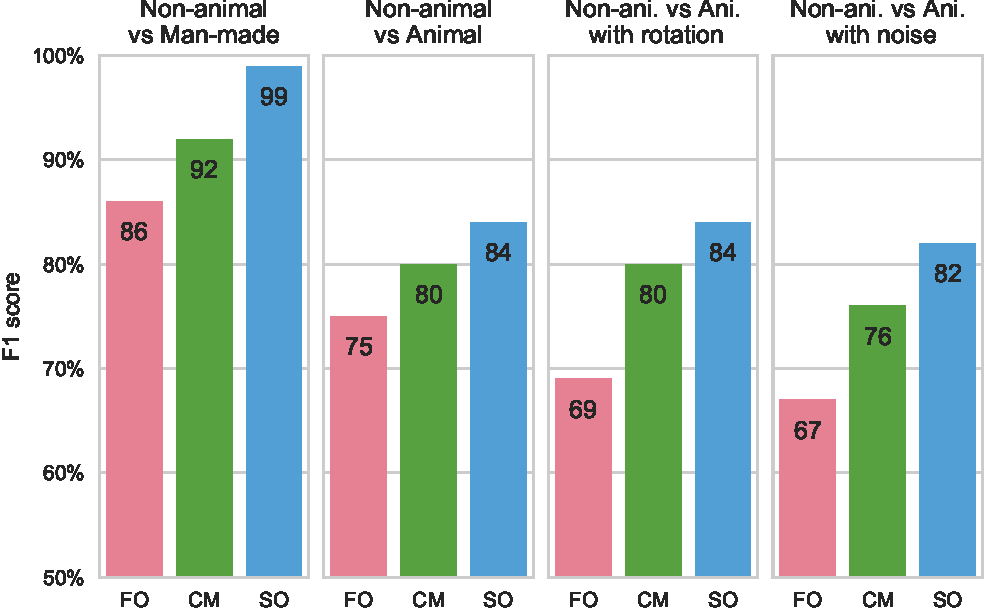
\includegraphics[width=.9\textwidth]{figure_results}%
\caption{%
Classification results. 
To quantify the difference in low-level feature statistics across categories (see Figure~\ref{fig:chevrons2}), we used a standard Support Vector Machine (SVM) classifier to measure how each representation affected the classifier's reliability for identifying the image category. 
For each individual image, we constructed a vector of features as either 
%
(FO) the histogram of first-order statistics as the histogram of edges'  orientations,
(CM) the ``chevron map'' subset of the second-order statistics, (i.e., the two-dimensional histogram of relative orientation and azimuth; see Figure~\ref{fig:chevrons}), or 
(SO) the full, four-dimensional histogram of second-order statistics (i.e., all parameters of the edge co-occurrences).
%
  We gathered these vectors for each different class of images and
  report here the results of the SVM classifier using an
  F1 score (50\% represents chance level).  While it was expected that differences would be clear between non-animal natural images versus
  laboratory (man-made) images, results are still quite high for
  classifying animal images versus non-animal natural images, and are in the range reported by~\citet{Serre07} (F1 score of 80\% for human observers and 82\% for their model), even 
using the CM features alone. %
\label{fig:results}}%
\end{figure}%
% -------------------------------- %
Note that by definition, our measure of the statistics of edge co-occurrence 
is invariant to translations, scalings, and rotations in the plane of the image.
This last property---not shared by first-order statistics of edges---makes it possible to explain the rather unintuitive result that
categorization in humans is relatively independent to rotations~\citep{Crouzet11b}. 
We also performed the same classification where images' %from both databases 
signal-to-noise ratio was halved (``+ Noise'' condition above). 
Results are degraded but qualitatively similar, as was also observed
in psychophysical experiments~\citep{Wichmann06}. 

Finally, if humans use edge co-occurences to do rapid image
categorization, images falsely detected by humans as containing
animals should have second-order statistics similar to those of images
that do contain animals.  Figure~\ref{fig:false-alarms} shows that the
set of the most common false-alarm images does have a chevron map
strikingly similar to that for images that do have animals, and that
on average the false alarm images have second-order histograms closer
to the animal than to the non-animal datasets.

% -------------------------------- %
%: fig:false-alarms
\begin{figure}%[p]%[ht!]
\centering%
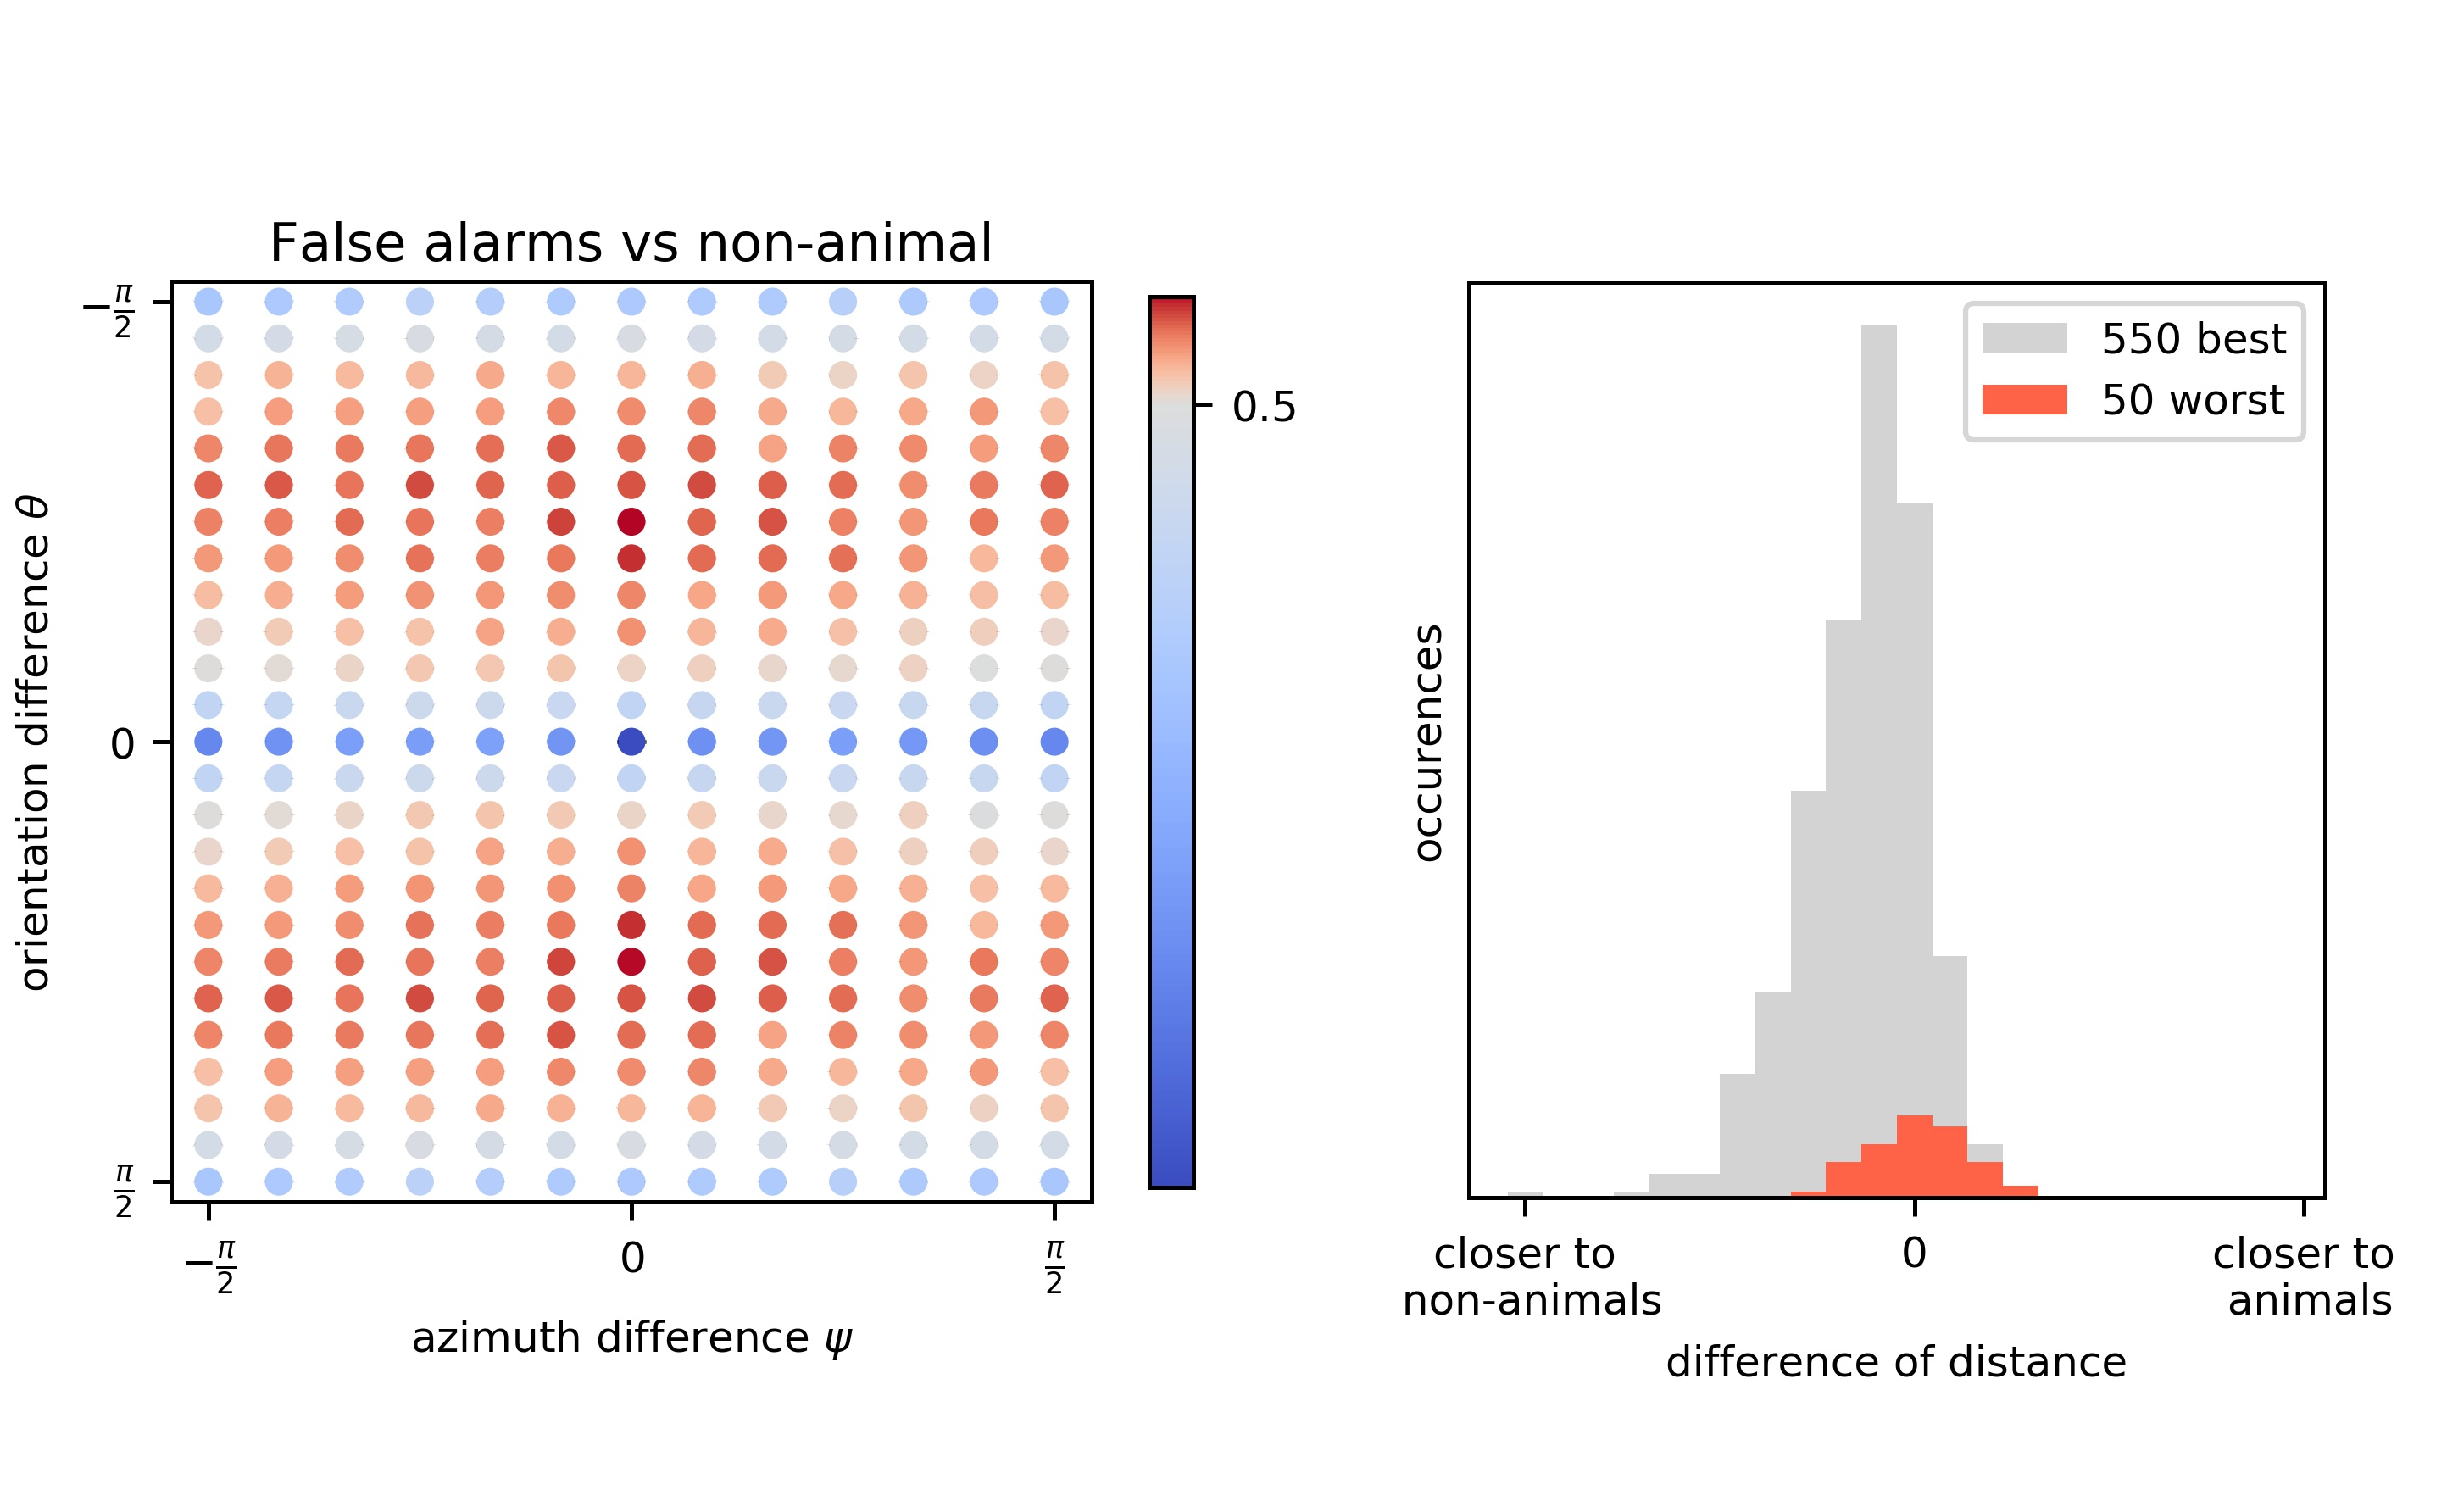
\includegraphics[width=.9\textwidth]{figure_FA_humans}%
\caption{%
  To see whether the patterns of errors made by humans are consistent
  with our model, we studied the second-order statistics of the 50
  non-animal images that human subjects in~\citet{Serre07} most
  commonly falsely reported as having an animal. We call this set of
  images the ``false-alarm image dataset''.  (Left) This chevron map
  plot shows the ratio between the second-order statistics of the
  false-alarm images and the full non-animal natural image dataset,
  computed as in Figure~\ref{fig:chevrons2} (left).  Just as for the
  images that actually do contain animals (Figure~\ref{fig:chevrons2},
  left), the images falsely reported as having animals have more
  co-circular and converging (red chevrons) and fewer collinear and
  orthogonal configurations (blue chevrons).  (Right) To quantify this
  similarity, we computed the Kullback-Leibler distance between the
  histogram of each of these images from the false-alarm image
  dataset, and the average histogram of each class. The difference
  between these two distances gives a quantitative measure of how
  close each image is to the average histograms for each class.
  Consistent with the idea that humans are using edge co-occurences to
  do rapid image categorization, the 50 non-animal images that were
  worst classified are biased toward the animal histogram ($d' = 1.04$),
  while the 550 best classified non-animal images are closer to the
  non-animal histogram.
\label{fig:false-alarms}}%
\end{figure}%
% -------------------------------- %
%}{\color{green}
%%%%%%%%%%%%%%%%%%%%%%%%%%%%%%%%%%%%%%%
\section*{Discussion} 
%%%%%%%%%%%%%%%%%%%%%%%%%%%%%%%%%%%%%%%
%%%%%%%%%%%%%%%%%%%%%%%%%%%%%%%%%%%%%%%

These results call into question previous claims that a hierarchical
analysis of the visual scene is necessary 
for classification into high-level categories~\citep{Serre07}. 
We speculate that the observed differences in second-order statistics for images
with animals have an underlying basis in the physical constraints 
governing the shapes of animals. 
Specifically, animals typically have compact shapes, constrained by
their capacity to move, unlike plants rooted
in one location that must stretch rather than move towards resources.
%The bodies of animals are also often enveloped by a flexible membrane, 
%which by the constraint of minimal surface area will tend to assume a circular shape, 
%just as a bubble will. 
Conversely, man-made objects tend to have long, straight lines due to
their methods of manufacture.  We would
expect that other categories of objects could similarly be
distinguished by their second-order statistics, assuming that their
form %of those objects
follows their function in ways analogous to the categories tested
here.  Thus we expect that the second-order statistics will be useful
as a rough but general and fast method for distinguishing a wide range
of scene and object categories.  Similar observations apply to other
sensory systems, where we would expect co-occurence between primary
sensory elements (such as stimulation of a patch of skin, presence of
a specific auditory frequency, or activation of a taste or smell
receptor) to differ between ecologically important classes of stimuli.

% round 2
   In this study, we showed that edge co-occurrences were sufficient
   to distinguish between the animal/non-animal datasets from
   \citet{Serre07} and \citet{Kirchner06}, with performance comparable
   to that of humans in rapid categorization tasks.  We also showed
   that these statistics can distinguish between these datasets and
   scenes of various man-made environments.  How well will this
   approach generalize to other datasets, such as different
   combinations of animal/non-animal datasets?  Our analysis suggests
   that similar performance should be found for all dataset pairs that
   have a statistically significant difference in the ``roundness'' of
   the contours extracted in the images.  Although we expect such
   differences to be found reliably across the animal/non-animal
   datasets currently in use, it should be possible to find or
   construct a non-animal dataset that has similar edge co-occurence
   statistics to that of an animal dataset. For such comparisons, the
   model predicts that human observers would also have trouble rapidly
   making such a distinction (as suggested by the similar patterns of
   errors in figure~\ref{fig:false-alarms}).  Selecting or constructing such image
   sets and testing them with human observers will be an important way
   that the performance of this approach can be tested in future
   studies; even though humans should be able to categorize the images
   reliably when given enough time for study, the model predicts that
   they will be unable to do so under the constraints of rapid
   categorization.

In addition, our results predict that animal measurements of $p(\theta,
\psi)$ should be dynamically adaptive, as recently reported
by~\citet{McManus11} for macaque V1, since 
$p(\theta, \psi)$ varies strongly across environments. 
  The statistics of the dense network of lateral connections in V1
  analyzed by~\citet{Bosking97} and~\citet{Hunt11} suggest that a
  local representation of these probabilities is available for
  supporting such computations.  We predict that if these patterns of
  connectivity are built by adapting to the visual statistics, e.g.,
  through Hebbian learning~\citep{Bednar12jpp}, lab-reared animals
  will have much stronger connections between neurons with collinear
  preferences than will wild-raised animals.
Finally, a straightforward prediction is 
that neural activity in early visual areas contributes
directly to making even seemingly high-level judgments.
Indeed, the model suggests that
this set of features could be computed locally in these areas and
projected to cortical or subcortical areas that mediate
fast behavioral responses~\citep{Rice14}.  This prediction could be tested using
methods similar to those in~\citet{Michel13}, by recording neural
activity in V1 in animals performing decision-making tasks with images
whose curvature distribution has been synthetically modified.
%%
%In particular, novel analysis of the data from~\citet{Bosking97}
%by~\citet{Hunt11} has suggested that co-circularity is weak but present, and
%also (surprisingly) that anti-cocircular edge co-occurrences may be connected.
%Indeed, an anti-circular arrangement is less-likely that normal, and therefore
%carries surprising information with respect to the model of smooth contours,
%possibly about contour disruption or the presence of corners. This confirms the
%idea of the brain as a generic information processing machine, but questions
%the actual information representation that may actually be used in the neural
%activity. %
%%%%%%%%%%%%%%%%%%%%%%%%%%%%%%%%%%%%%%
%%%%%%%%%%%%%%%%%%%%%%%%%%%%%%%%%%%%%%
%% Optional Materials and Methods Section
%% The Materials and Methods section header will be added automatically.
%
%% Enter any subheads and the Materials and Methods text below.
%\section{Methods}
%}
\section*{Methods Summary} %: Materials text  189 words
%%%%%%%%%%%%%%%%%%%%%%%%%%%%%%%%%%%%%%
%---------------------------------------------------------------------------%
The first step of our method involves defining the dictionary of templates or
filters for detecting edges. 
We use a log-Gabor representation, which is well suited to represent 
a wide range of natural images~\citep{Fischer07} (animal or non-animal). 
This representation gives a generic model of edges as defined by their shape,
orientation, and scale. 
We set the parameters to match what has been reported 
for simple-cell responses in macaque area V1. 
This architecture is similar to that used by~\citet{Geisler01} 
and is detailed in the supplementary material. 

The resulting dictionary of edge filters is over-complete. 
The linear representation would thus give an inefficient representation 
of the distribution of edges (and thus of the statistics of edge co-occurrences).
Therefore, starting from this linear representation, 
we searched for the most sparse representation.
Because this search is combinatorial and thus very computationally
expensive, we approximated a solution using a greedy approach first
proposed by~\citet{Perrinet02sparse}.
%
To validate the categorization performance, 
we used the standard SVM library as implemented by~\citet{Pedregosa11}. 
We used the Jensen--Shannon divergence distance
as a metric between histograms~\citep{Cha02}. %, 
The results of the SVM classifier are given as the F1 score
to directly compare our method to that of~\citet{Serre07}.
%
\bibliographystyle{unsrtnat}%plainnat}%
\bibliography{../bib/PerrinetBednar15}

%\subsection*{Acknowledgments}  %
\subsection*{Additional Information}  %
The authors declare no competing financial interests.

\noindent\Acknowledgments %
\subsection*{Author contribution statement}  %
L.U.P. and J.A.B. wrote the main manuscript text and L.P. prepared figures. All authors reviewed the manuscript. 
\includepdf[pages=-]{PerrinetBednar15supplementary.pdf}
\end{document}%
